% preâmbulo: \usepackage{tikz}  \usepackage{subcaption}
\definecolor{cgreen}{RGB}{0,153,0}
\definecolor{cred}{RGB}{204,0,0}
\definecolor{cblue}{RGB}{0,114,220}
\definecolor{cpurple}{RGB}{128,0,128}
\definecolor{cbrown}{RGB}{120,63,20}
\definecolor{cpink}{RGB}{255,160,160}
\definecolor{cyellow}{RGB}{240,210,0}

\begin{figure}[htb]
  \centering
  \begin{subfigure}[b]{0.52\textwidth}
    \centering
    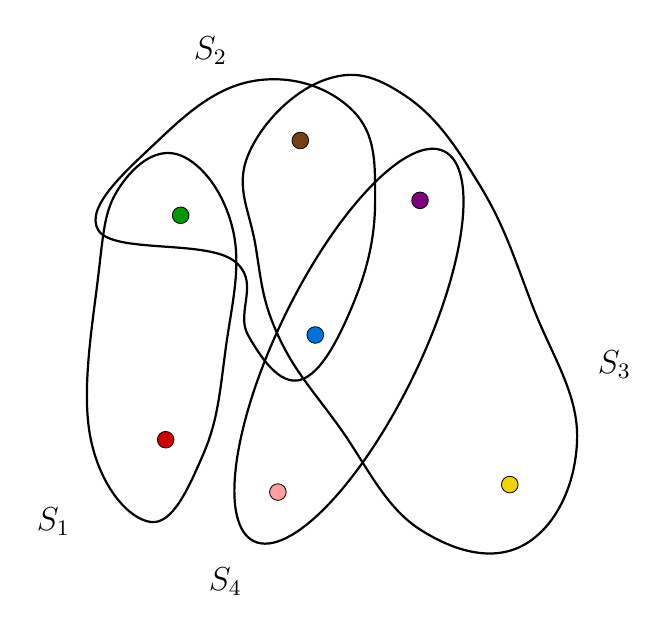
\begin{tikzpicture}[scale=0.95,
        elt/.style={circle,draw=black,line width=0.3pt,inner sep=0pt,minimum size=6pt},
        setlab/.style={font=\large}]

      \draw[line width=0.8pt] plot[smooth cycle,tension=0.7]
        coordinates {(0.6,4.0) (1.3,3.0) (1.2,1.4) (0.9,0.0) (0.2,-0.9)
                     (-0.6,0.2) (-0.5,2.4) (-0.2,3.6)};                 % S1
      \draw[line width=0.8pt] plot[smooth cycle,tension=0.7]
        coordinates {(-0.5,3.0) (0.3,4.2) (1.6,5.0) (2.9,4.6) (3.2,3.4)
                     (2.9,2.0) (2.2,1.0) (1.5,1.6) (1.3,2.6)};          % S2
      \draw[line width=0.8pt] plot[smooth cycle,tension=0.7]
        coordinates {(2.5,5.0) (1.5,4.0) (1.6,2.8) (1.9,1.6) (2.7,0.4)
                     (3.8,-1.0) (5.2,-1.2) (5.9,0.2) (5.3,2.0) (4.6,3.6)
                     (3.6,4.8)};                                        % S3
      \draw[line width=0.8pt,rotate around={64:(2.85,1.45)}]
        (2.85,1.45) ellipse (2.9 and 0.95);                             % S4

      \node[elt,fill=cgreen]  at (0.6,3.2)  {};
      \node[elt,fill=cbrown]  at (2.2,4.2)  {};
      \node[elt,fill=cpurple] at (3.8,3.4)  {};
      \node[elt,fill=cblue]   at (2.4,1.6)  {};
      \node[elt,fill=cred]    at (0.4,0.2)  {};
      \node[elt,fill=cpink]   at (1.9,-0.5) {};
      \node[elt,fill=cyellow] at (5.0,-0.4) {};

      \node[setlab] at (-1.1,-0.9) {$S_1$};
      \node[setlab] at (1.0,5.4)   {$S_2$};
      \node[setlab] at (6.4,1.2)   {$S_3$};
      \node[setlab] at (1.2,-1.7)  {$S_4$};
    \end{tikzpicture}
    \caption{Instance of set cover.}
    \label{fig:reduction-set-cover}
  \end{subfigure}
  \hfill
  \begin{subfigure}[b]{0.44\textwidth}
    \centering
    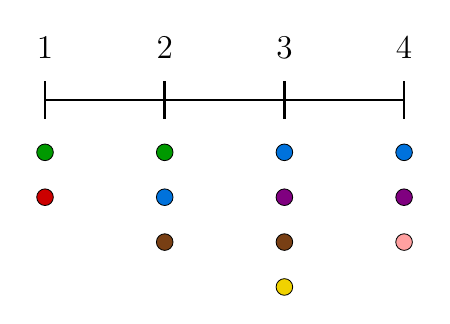
\begin{tikzpicture}[scale=0.95,
        elt/.style={circle,draw=black,line width=0.3pt,inner sep=0pt,minimum size=6pt}]
      \draw[line width=0.8pt] (0,2.6) -- (4.8,2.6);
      \foreach \x/\lab in {0/1, 1.6/2, 3.2/3, 4.8/4} {
        \draw[line width=1pt] (\x,2.35) -- (\x,2.85);
        \node[font=\large] at (\x,3.3) {$\lab$};
      }
      \foreach \c [count=\i from 0] in {cgreen,cred}
        \node[elt,fill=\c] at (0,{1.9-0.6*\i}) {};
      \foreach \c [count=\i from 0] in {cgreen,cblue,cbrown}
        \node[elt,fill=\c] at (1.6,{1.9-0.6*\i}) {};
      \foreach \c [count=\i from 0] in {cblue,cpurple,cbrown,cyellow}
        \node[elt,fill=\c] at (3.2,{1.9-0.6*\i}) {};
      \foreach \c [count=\i from 0] in {cblue,cpurple,cpink}
        \node[elt,fill=\c] at (4.8,{1.9-0.6*\i}) {};
    \end{tikzpicture}
    \caption{Corresponding colorful $k$-center instance.}
    \label{fig:reduction-colorful}
  \end{subfigure}
  \caption{Example of the reduction. In~\subref{fig:reduction-set-cover}, an
  instance of set cover with $U$ consisting of seven elements, each drawn as a
  distinct color, and $\mathcal{S} = \{S_1,S_2,S_3,S_4\}$.
  In~\subref{fig:reduction-colorful}, for each $i \in [s]$, the elements of
  $S_i$ become points of the respective colors placed at position $i$ of the
  real line.}
  \label{fig:reduction-set-cover-colorful}
\end{figure}